% Seção: Dados
% Dono: Miguel · Orçamento: 1 página(s) · docs/fontes/plano-de-projeto.md §14.1
% Conteúdo: Fonte, limpeza, recorte e estatísticas da rede
\section{Dados}\label{sec:dados}

O projeto usa o GTFS convencional publicado pela Prefeitura de Belo Horizonte
(\url{https://dados.pbh.gov.br/dataset/gtfs}). O instantâneo baixado em 05/11/2026
foi identificado pelo SHA-256 iniciado em \texttt{623bdf422fb0}; o valor
completo está no arquivo da feature P0-DADOS.
O script de download registra origem e data fora do Git para permitir reproduzir
as medições com o mesmo arquivo.

O leitor converte paradas, linhas, viagens, horários e calendário em uma rede
normalizada. Seleciona uma quarta-feira ativa, aplica as exceções de
\texttt{calendar\_dates.txt}, conserva os horários por viagem e relata linhas
inválidas. A leitura de \texttt{stop\_times.txt} é feita em fluxo. Um recorte por
caixa geográfica ou linhas preserva apenas trechos consecutivos, sem criar uma
ligação direta onde uma parada intermediária foi removida. A
Figura~\ref{fig:atividade-dados} resume o processamento.

\begin{figure}[ht]
  \centering
  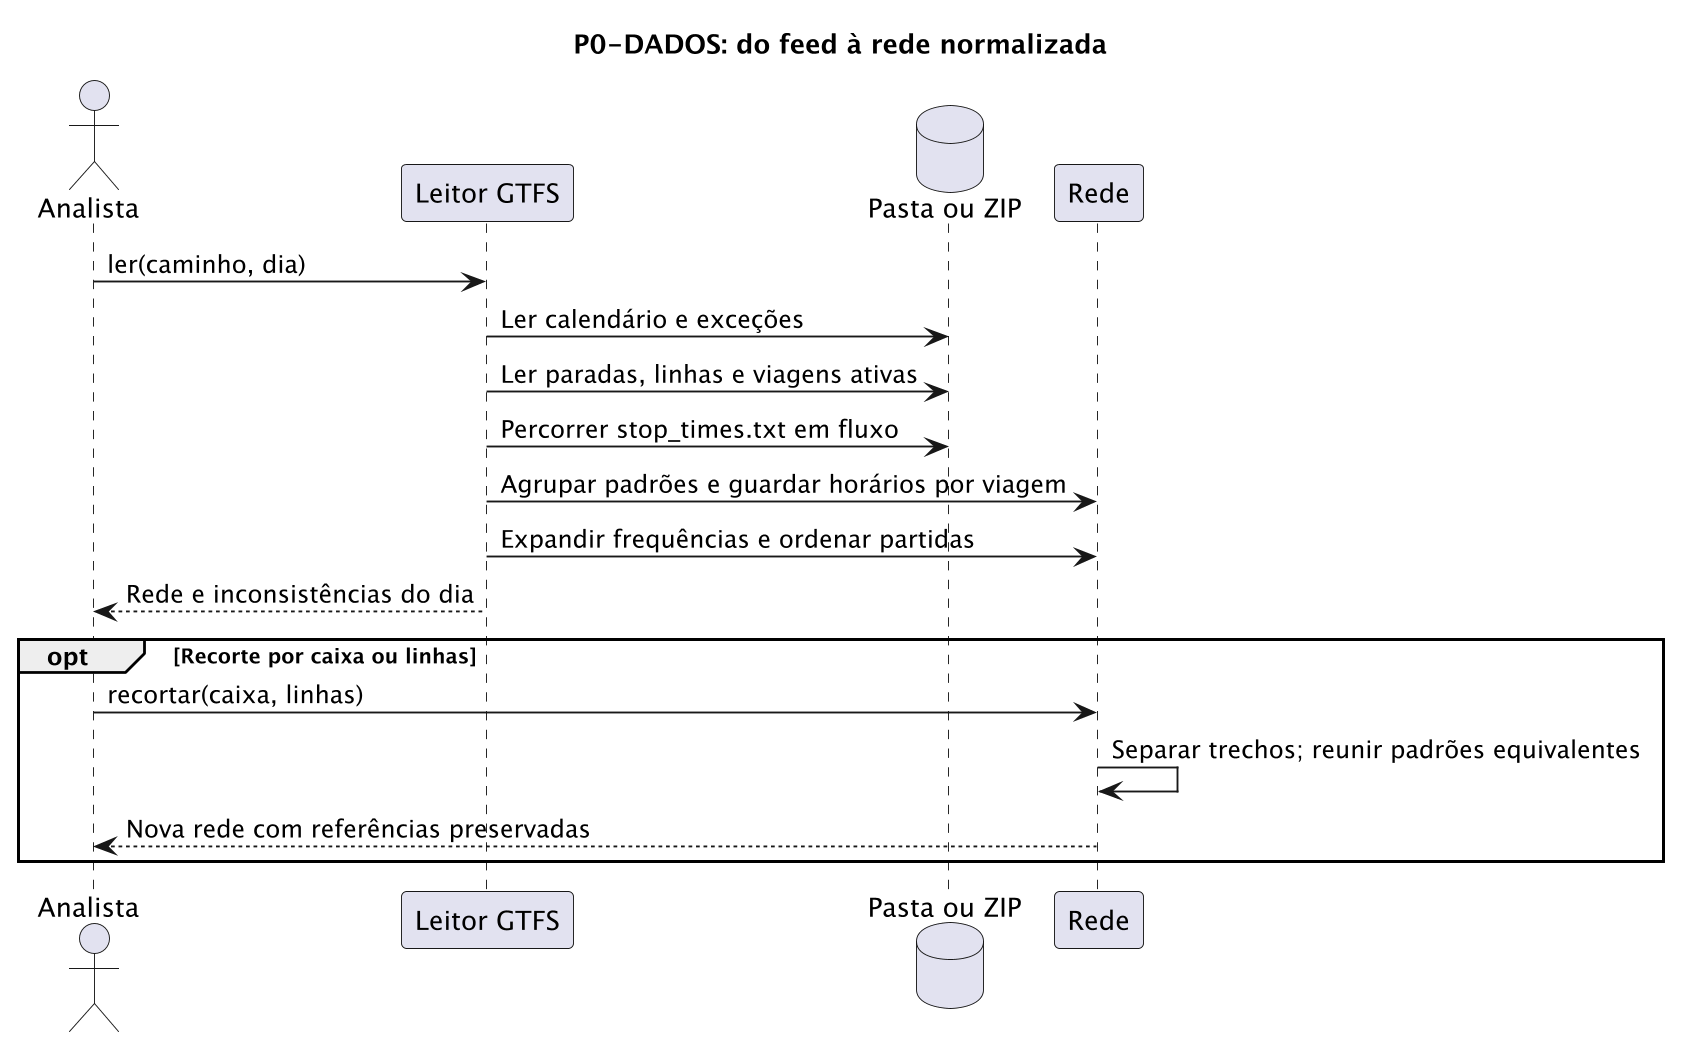
\includegraphics[width=0.82\linewidth]{sequencia-dados-resumo.png}
  \caption{Leitura e recorte do GTFS até a rede normalizada.}
  \label{fig:atividade-dados}
\end{figure}

No serviço de 04/11/2026, a execução de \texttt{ler("dados/brutos/bhtrans.zip")}
produziu 9.659 paradas, 303 linhas, 698 padrões e 24.503 viagens. O leitor não
reportou inconsistências para esse serviço. A leitura foi medida com
\texttt{medir(ler, caminho, repeticoes=3)}: média de 7,753~s e desvio amostral
de 0,114~s em MacBook Air com Apple M4, 16~GB e Python~3.14.6. Esses valores
descrevem o modelo de dados; o número de arestas só existe após construir uma
visão de grafo. A validação atual examina o dia selecionado, não todas as datas
de vigência do feed.
